\chapter{Thiết kế hệ thống phân loại tự động}
\paragraph{Giới thiệu} Nội dung chương này sẽ tập trung vào cách mà chúng em tổ chức dữ liệu của hệ thống, cách áp dụng một số design pattern vào việc xây dựng hệ thống, các phác thảo sơ khai của giao diện, cách sử dụng kết hợp các thư viện lập trình đã giới thiệu vào Vaadin Framework và cuối cùng là thiết kế một ontology dùng để trình bày tính năng phân loại sau khi hệ thống được xây dựng thành công. Đầu tiên, chúng em xin mô tả bố cục của giao diện.
\section{Giao diện phác thảo}
\begin{figure}[ht!]
	\centering
	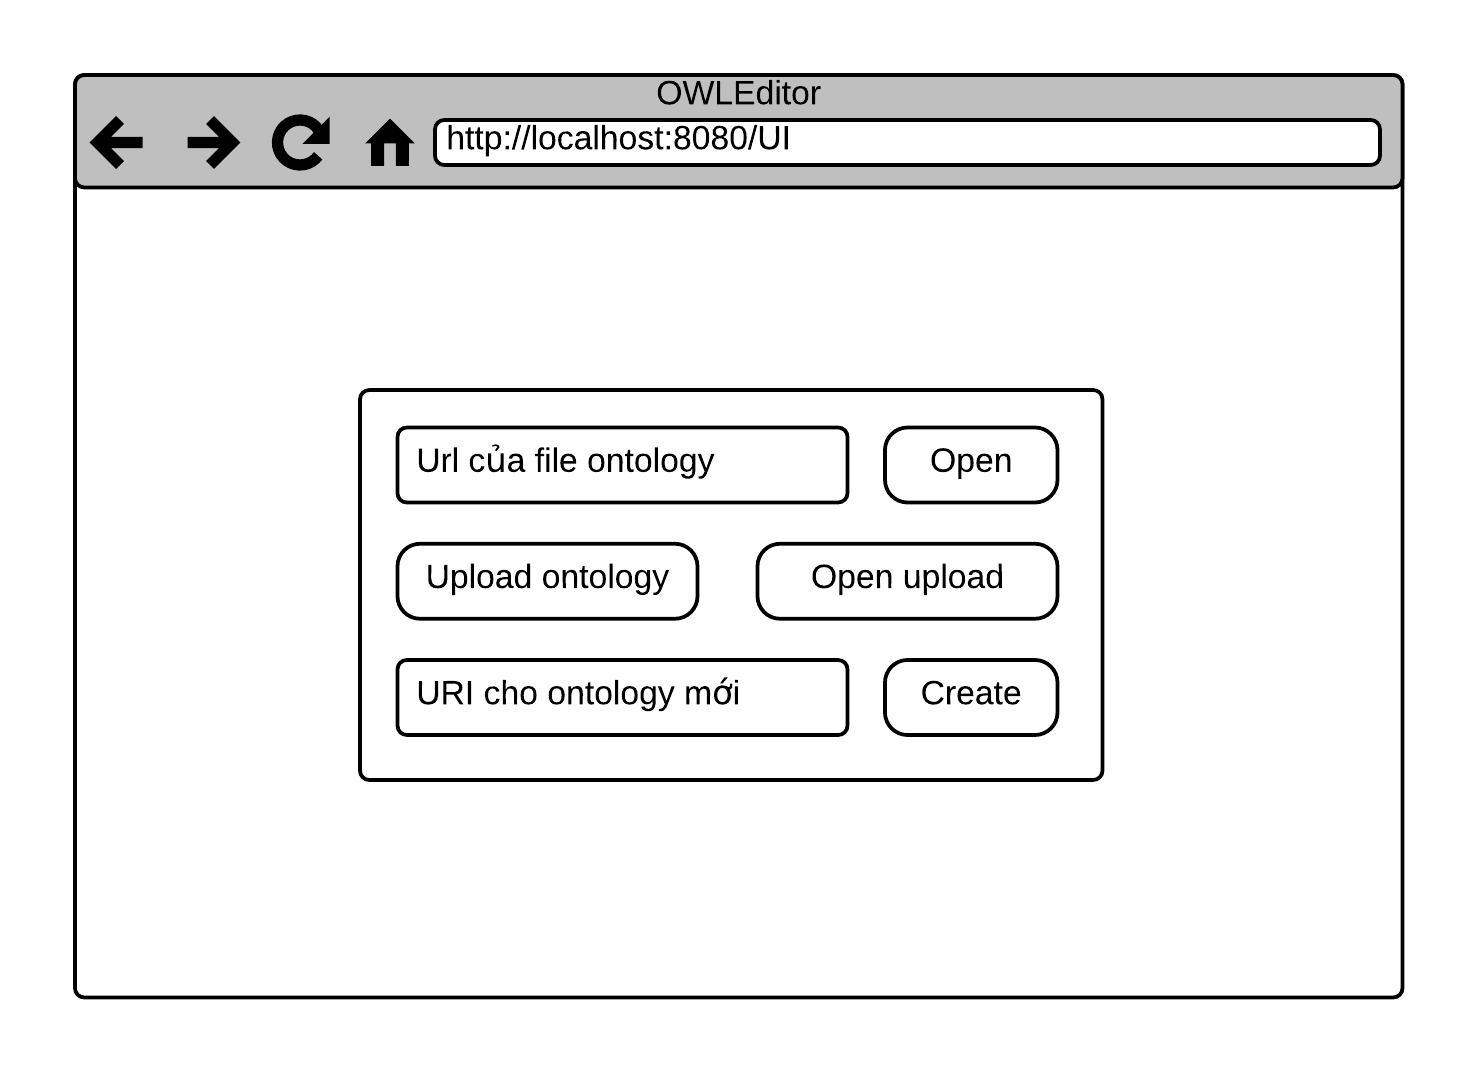
\includegraphics[width=130mm]{Figures/ui_entryview.png}
	\caption{Phác thảo Entry View \label{overflow}}
\end{figure}
Hệ thống hay ứng dụng sẽ gồm 2 view chính: view đầu tiên tạm gọi là EntryView dùng để nạp/tạo mới các tài liệu OWL 2. View thứ hai chính là view chính của ứng dụng gọi làm MainView cho phép thực hiện việc chỉnh sửa ontology, thực hiện suy luận (phục vụ cho tính năng phân loại). 
\\
MainView sẽ gồm nhiều tab, mỗi loại thực thể (gồm lớp, thuộc tính đối tượng, thuộc tính dữ liệu, cá thể) và SWRL Rule sẽ được tổ chức thành từng tab với tên tương ứng. 
\begin{figure}[h!]
	\centering
	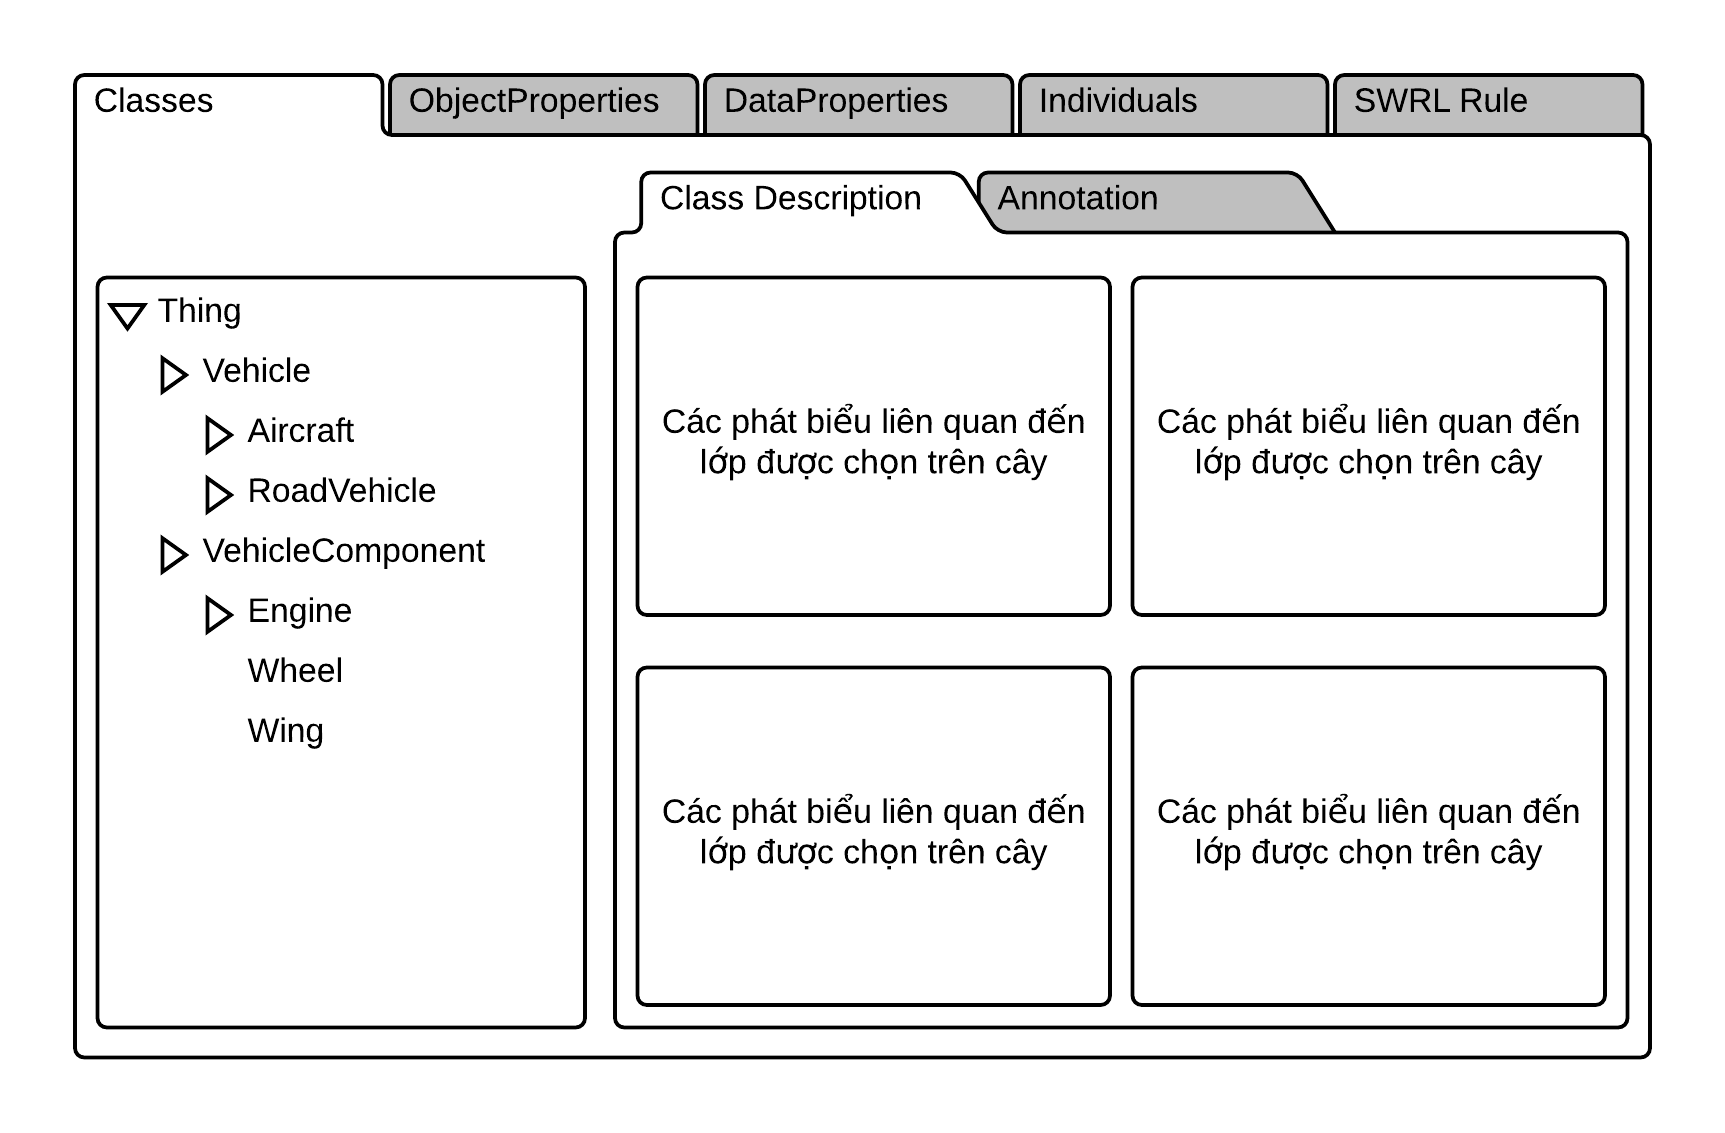
\includegraphics[width=150mm]{Figures/ui_mainview.png}
	\caption{Phác thảo Main View - Tab "Classes" (chứa lớp và các mô tả lớp liên quan) \label{overflow}}
\end{figure}
\begin{figure}[h!]
	\centering
	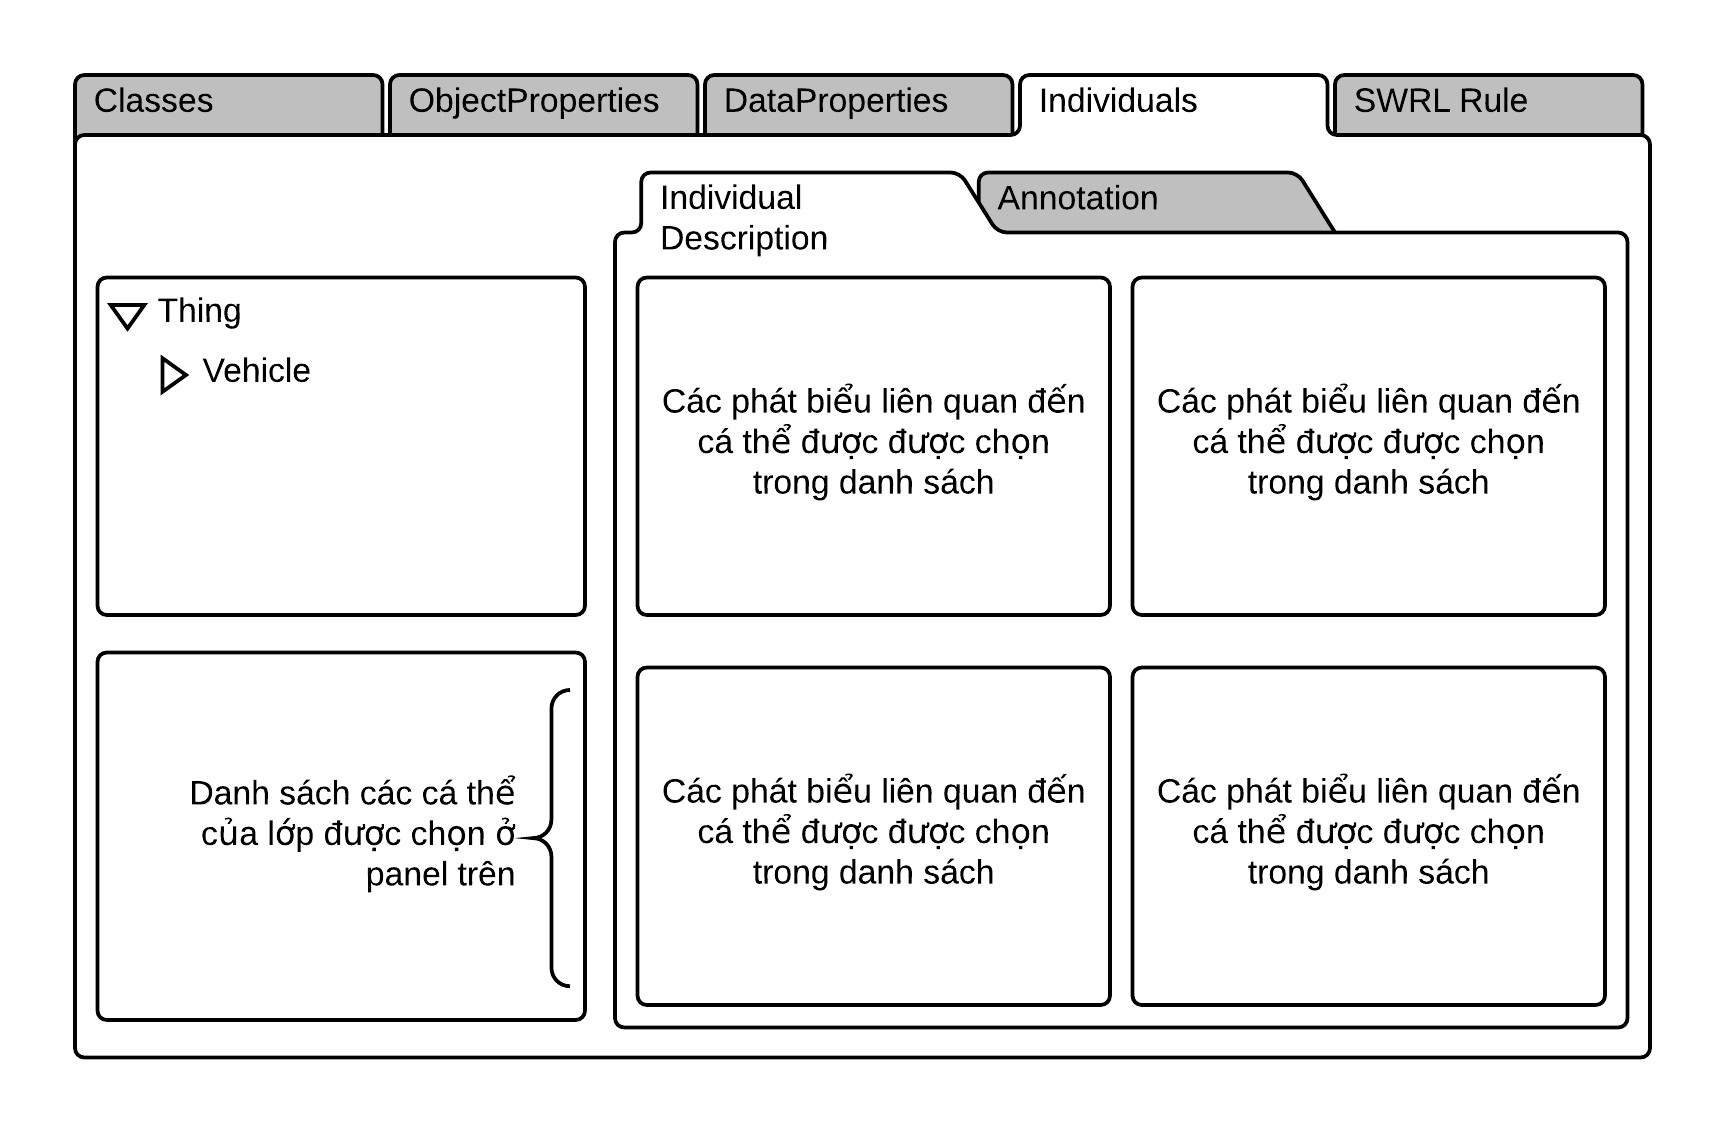
\includegraphics[width=150mm]{Figures/ui_mainview_individual.png}
	\caption{Phác thảo Main View - Tab "Individuals" (chứa cá thể và các mô tả liên quan) \label{overflow}}
\end{figure}
\begin{figure}[ht!]
	\centering
	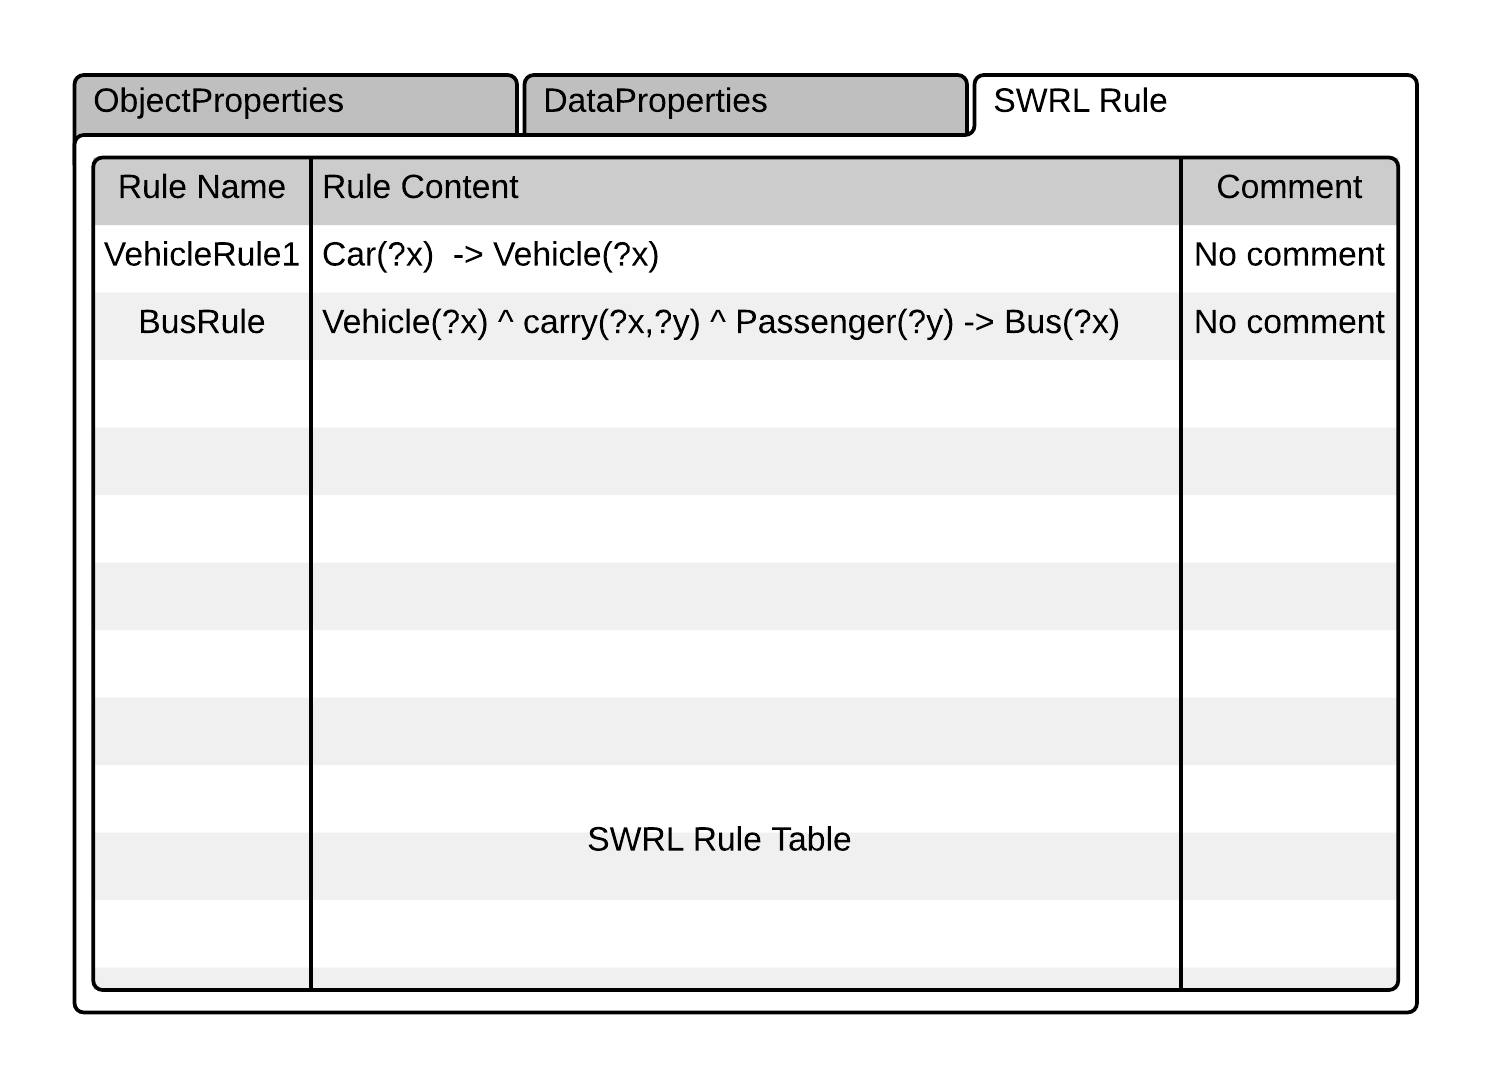
\includegraphics[width=140mm,height=95mm]{Figures/ui_mainview_swrltab.png}
	\caption{Phác thảo Main View - Tab "SWRL Rules" \label{overflow}}
\end{figure}
Các tab về lớp, thuộc tính đối tượng và dữ liệu sẽ có bố cục giống nhau (Hình 3.2), với bên trái là một cây biểu diễn cấu trúc phân cấp của các loại thực thể này và bên phải là các panel nhỏ. Từng panel sẽ tương ứng với từng loại phát biểu có liên quan đến thực thể được chọn bên trái. Riêng tab về các cá thể sẽ có bố cục hơi khác so với các thực thể còn lại, nó sẽ có thêm một danh sách (sẽ nằm bên dưới cấu trúc cây chứa các lớp - Hình 3.3). Bên trong tab SWRL Rules sẽ là một bảng gồm chứa các rule, chia thành 3 cột gồm tên, nội dung và lời chú thích cho rule (Hình 3.4).
\begin{figure}[h!]
	\centering
	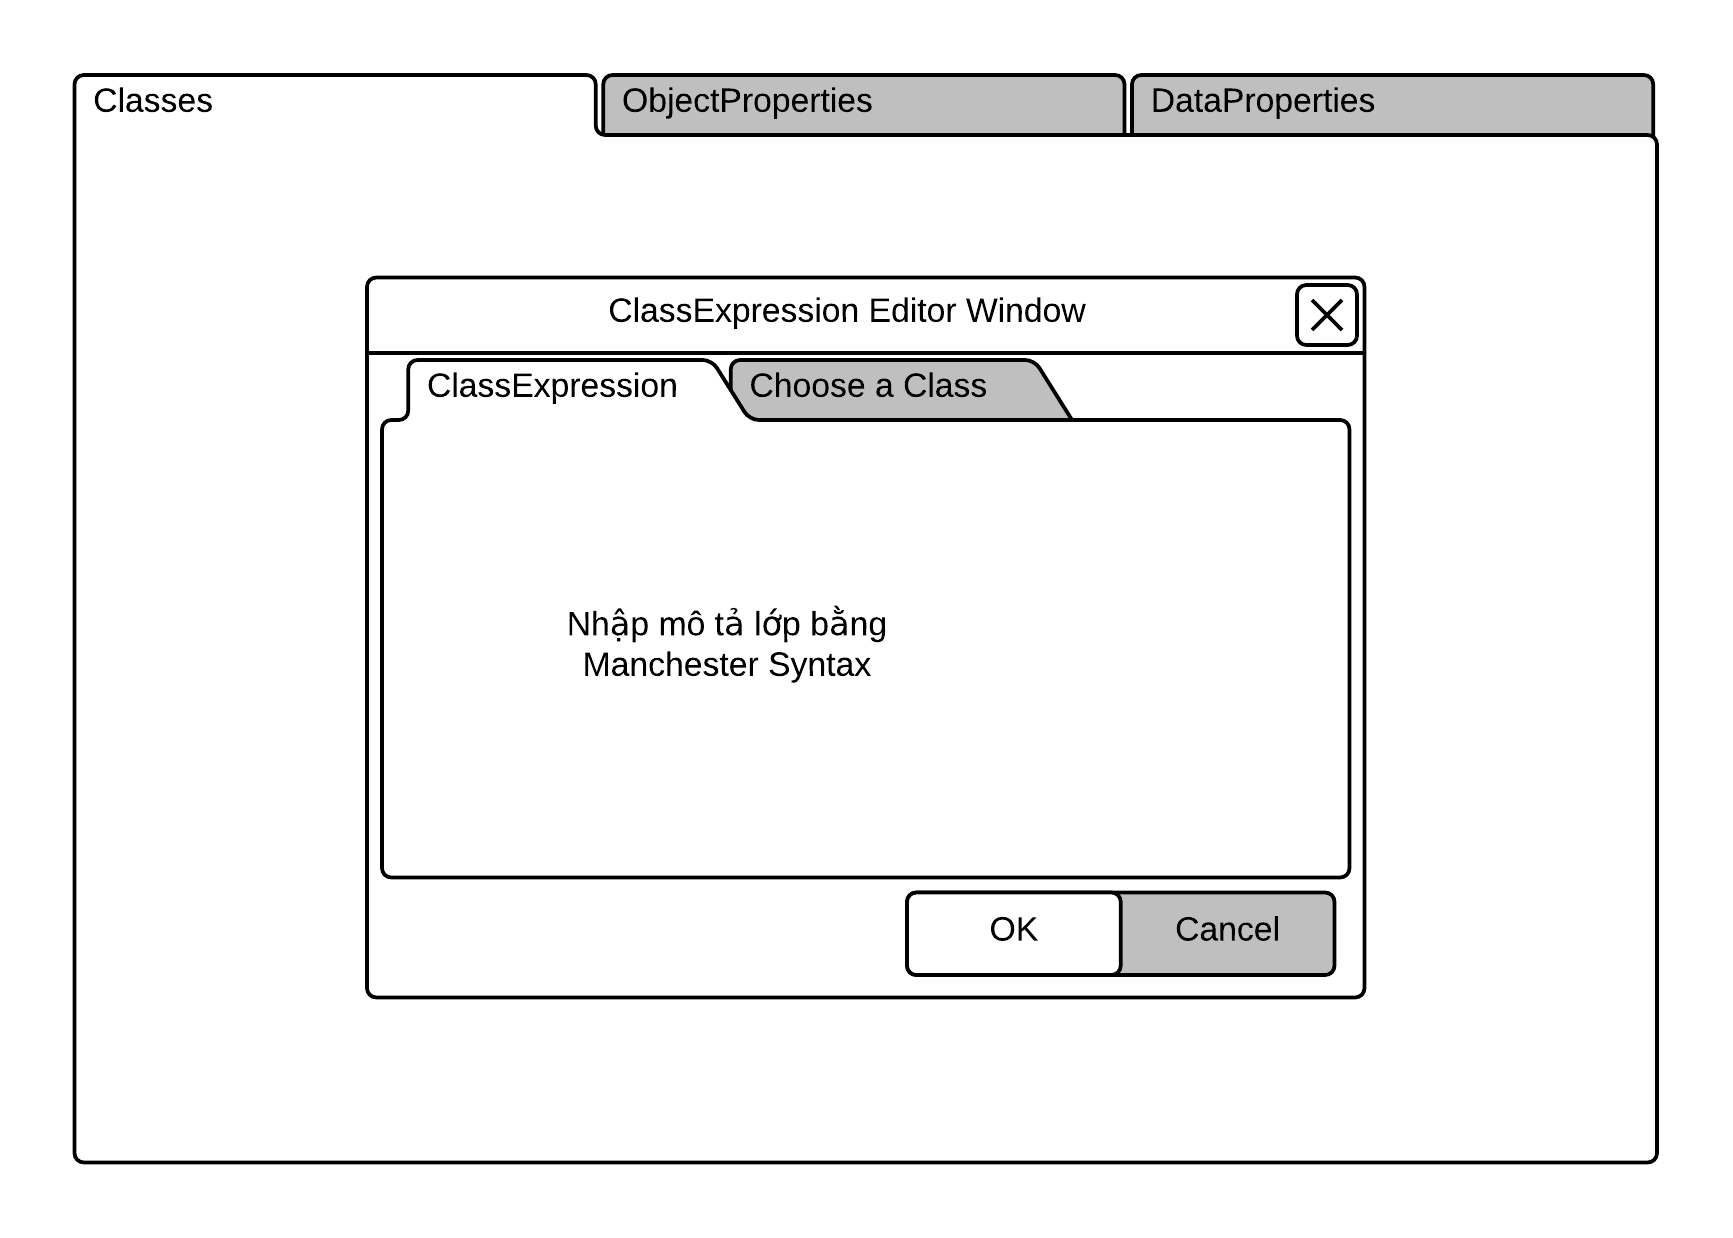
\includegraphics[width=150mm]{Figures/ui_classexpressioneditor.png}
	\caption{Phác thảo cửa sổ biên tập mô tả lớp\label{overflow}}
\end{figure}
\begin{figure}[h!]
	\centering
	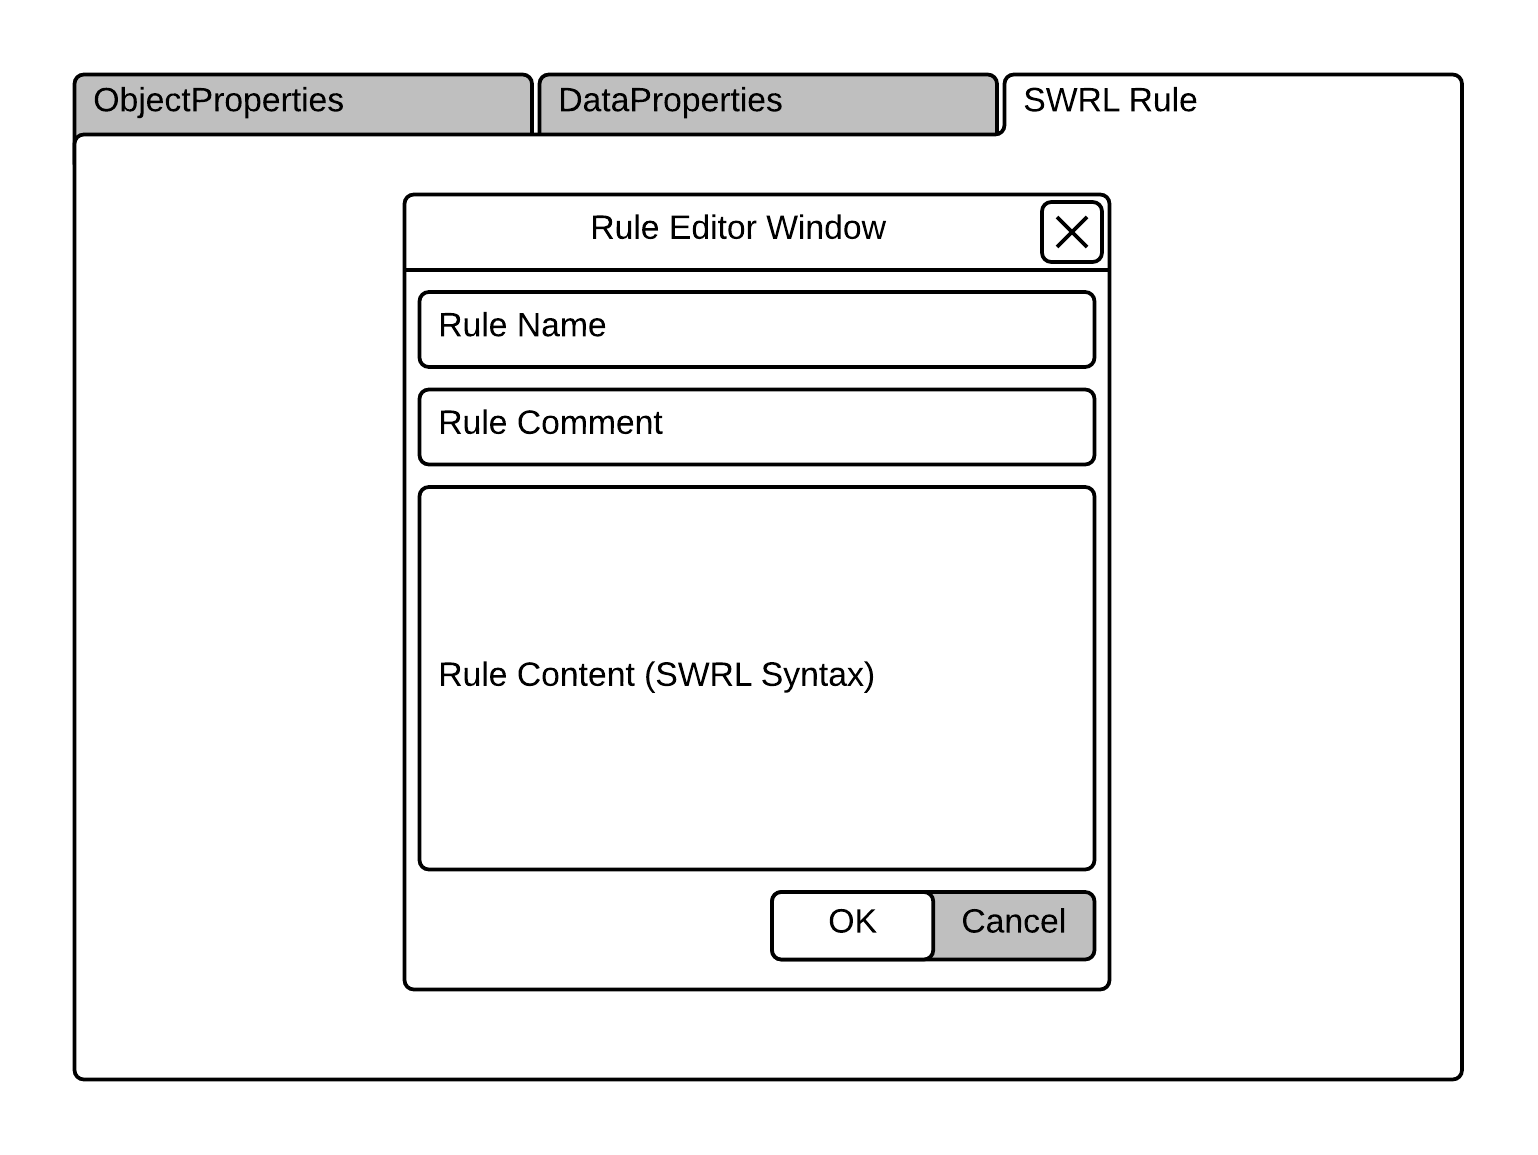
\includegraphics[width=150mm,height=100mm]{Figures/ui_mainview_ruleeditor.png}
	\caption{Phác thảo cửa sổ biên tập rule \label{overflow}}
\end{figure}
Ngoài các view và tab đã kể ở trên, thì ứng dụng buộc phải có thêm các thành phần giao diện hỗ trợ viêc biên tập mô tả lớp, thuộc tính, cá thể (class/property expression, individual assertion axiom) và việc biên tập SWRL Rule. Các hình sau thể hiện phác thảo về các giao diện đảm nhiệm những tính năng vừa nêu.